\PassOptionsToPackage{table}{xcolor}
\documentclass[pdf]{beamer}
\mode<presentation>{\usetheme{Dresden}}
\usepackage{lmodern}
\usepackage[normalem]{ulem}
\usepackage{amsmath,textcomp,amssymb,geometry,graphicx,listings,array,color,amsthm}
\usepackage{pgfplots}

\usepackage[noend]{algpseudocode}

\usepackage[
backend=biber,
sorting=ynt,
]{biblatex}
\addbibresource{lecture.bib}

\usepackage{tikz}
\usepackage{multicol}
\usetikzlibrary{shapes,snakes}
\usetikzlibrary{positioning}
\usetikzlibrary{arrows}
\usetikzlibrary{fit}
\usetikzlibrary{math}

%% For on-slide alerting of nodes
\tikzstyle{alert} = [text=black, fill=blue!20, draw=black]
\setbeamercolor{alerted text}{fg=blue}
\tikzset{alerton/.code args={<#1>}{%
  \only<#1>{\pgfkeysalso{alert}} % \pgfkeysalso doesn't change the path
}}

%% utils for removing uninteresting sections from the navbar
%% https://tex.stackexchange.com/questions/317774/hide-section-from-sidebar
\makeatletter
\let\beamer@writeslidentry@miniframeson=\beamer@writeslidentry%
\def\beamer@writeslidentry@miniframesoff{%
  \expandafter\beamer@ifempty\expandafter{\beamer@framestartpage}{}% does not happen normally
  {%else
    % removed \addtocontents commands
    \clearpage\beamer@notesactions%
  }
}
\newcommand*{\miniframeson}{\let\beamer@writeslidentry=\beamer@writeslidentry@miniframeson}
\newcommand*{\miniframesoff}{\let\beamer@writeslidentry=\beamer@writeslidentry@miniframesoff}
\makeatother

%% preamble
\title{Chebyshev Picard Iteration}
\subtitle{Fixed Point IVP Integration}
\author{A.C.}
\date{\today}

\AtBeginSection[]
{
  \miniframesoff
  \begin{frame}{Outline}
    \tableofcontents[currentsection,hideothersubsections]
  \end{frame}
  \miniframeson
}

\definecolor{darkred}{rgb}{0.7,0,0}
\definecolor{darkgreen}{rgb}{0,0.5,0}
\definecolor{darkblue}{rgb}{0,0,0.5}
\definecolor{darkpurple}{rgb}{0.4, 0.0, 0.4}

%% Code font settings
\lstset{
  showstringspaces=false,
  basicstyle=\scriptsize\ttfamily,
  commentstyle=\color{darkred},
  stringstyle=\color{darkgreen},
  keywordstyle=\bfseries\color{darkpurple},
}

%%%%%%%%%%%%%%%%%%%%%%%%%%
% Start of Actual slides %
%%%%%%%%%%%%%%%%%%%%%%%%%%
\begin{document}
\begin{frame}
  \titlepage
\end{frame}

\section{Chebyshev Polynomials}

\subsection{Definition and Recurrence}

\begin{frame}{Starting Point}

  Consider:
   
  \[ \cos n \theta \]

  How does this relate to $\cos \theta$?
\end{frame}

\begin{frame}{$n+1$}

\begin{align*}
  \cos 0 &= 1\\
  \cos \theta &= \cos \theta\\
  \cos 2\theta &= 2\cos^2 \theta - 1\\
   & \vdots\\
  \cos (n+1)\theta &= 2 \cos \theta \cos n\theta - \cos (n-1)\theta\\
\end{align*}

See notes for proof.
  
\end{frame}

\begin{frame}{Recurrence}

Let $T_n(\cos \theta) := \cos n \theta$ and $x := \cos \theta$ and observe the following recurrence

\begin{align*}
  T_0 &= 1\\
  T_1 &= x\\
  T_{n+1} &= 2xT_n - T_{n-1}\\
\end{align*}

In closed form: $T_n(x) = \cos n \cos^{-1} x$

\end{frame}

\begin{frame}{Polynomial}
  \[ T_{n+1} = 2xT_n - T_{n-1} \]

  $2x$ multiplier increases degree of each subsequent $T_n$ by exactly one.
  Easy to see that $\{T_0, T_1, \ldots, T_n \}$ spans forms a basis set for
  $\mathbb{P}_n$.\newline

  More directly, we can find coefficients $c_0, c_1, \ldots, c_n$ for any
  polynomial $p_n$ s.t.

  \[ p_n = c_0T_0 + c_1T_1 + \cdots + c_nT_n \]
\end{frame}

\begin{frame}{Domain}
  The recurrence form of Chebyshev polynomials (of the first kind) applies
  across the whole real line.\newline

  The cosine form requires we restrict ourselves to the interval $[-1,1]$.\newline

  We will take it as a given that we are in the range $[-1,1]$ throughout.
\end{frame}

\subsection{Integration}

\begin{frame}{Integral}
  \begin{center}
    \[ \int T_k = \frac{1}{k+1} T_{k+1} - \frac{1}{k-1} T_{k-1} + C\]
  \end{center}
  For $k=0, k=1$, there are special cases:

  \begin{center}
    \[ \int T_0 = T_1 \]
    \[ \int T_1 =  \frac{1}{4}(T_0 + T_2) \]
  \end{center}


  See notes for proof.
\end{frame}


\begin{frame}{Key Result}
  If we have a polynomial in Chebyshev-space, then we can integrate it easily
  without changing basis (e.g. to the ``usual'' basis $1, x, x^2,\ldots$, where
  integration is even simpler).
\end{frame}

\subsection{Interpolation and Orthogonality}

\begin{frame}{Lagrange Interpolation}
  Recall: a polynomial of degree $n$ is uniquely determined by $n+1$ points $(x_0, y_0),\ldots,(x_n, y_n)$.\newline

  Langrange interpolation is a standard method for constructing such a polynomial:
  \[ p_n(x) = \sum_i y_i \prod_{j \neq i} \frac{x - x_j}{x_i - x_j} \]

  What if we would like the polynomial in terms of the Chebyshev basis?
\end{frame}


\begin{frame}{System of Equations}
  Given points $(x_0, y_0),\ldots,(x_n, y_n)$, can write and solve a system of equations

  \begin{align*}
  c_0T_0(x_0) + c_1T_1(x_0) + \cdots + c_nT_n(x_0) &= y_0\\
  c_0T_0(x_1) + c_1T_1(x_1) + \cdots + c_nT_n(x_1) &= y_1\\
   & \vdots\\
  c_0T_0(x_n) + c_1T_1(x_n) + \cdots + c_nT_n(x_n) &= y_n\\
  \end{align*}

  Fairly heavyweight computation, would prefer a cheaper solution.
\end{frame}

\begin{frame}{Orthogonality}
  Define

  \[ \langle f, g \rangle = \int_{-1}^1 \frac{1}{\sqrt{1-x^2}}fg \,dx \]

  It can be shown that
  
  \[ \langle T_j, T_k \rangle = \left\{
    \begin{array}{ll}
        0, & \text{if } j \neq k\\
        \pi, & \text{if } j = k = 0\\
        \frac{\pi}{2}, & \text{if } j = k > 0
    \end{array}
  \right.
  \]

  That is, Chebyshev polynomials form an \emph{orthogonal} basis
  over $\mathbb{P}_n$. See notes for proof.
\end{frame}


\begin{frame}{Inner Product Interpolation}
  Consider the equation

  \[ p_n = c_0T_0 + c_1T_1 + \cdots + c_nT_n \]

  Take the inner product against $T_k$ on each side to see

  \[ \langle p_n, T_k \rangle = c_k \langle T_k, T_k \rangle \]

  If we can compute $\langle p_n, T_k \rangle$ efficiently, then we have a fast
  procedure for acquiring the polynomial in Chebyshev form.
\end{frame}

\begin{frame}{Quadrature}
  It is far from obvious but Lobatto quadrature at
  Chebyshev nodes $x_j = \cos \frac{j\pi}{n}$ computes $\langle p_n, T_k \rangle$ exactly,
  giving us the formula

  \[ \langle p_n, T_k \rangle = \frac{\pi}{n} \sideset{}{''}\sum_j p_n\left(\cos \frac{j\pi}{n}\right) T_k\left(\cos \frac{j\pi}{n}\right) \]

  See notes for proof.
\end{frame}

\begin{frame}{Key Result}
  If we choose to interpolate a function $f$ at $n+1$ Chebyshev nodes, then the
  Chebyshev form of the resulting polynomial may be efficiently computed through
  simple sums.
\end{frame}

\subsection{Approximation Error}

\begin{frame}{Weierstrass Approximation Theorem}
  Given any smooth function $f$ on a compact interval $[a,b]$ and an arbitrary
  error tolerance $\epsilon$, there exists a polynomial $p$ s.t.

  \[ ||p - f||_\infty \leq \epsilon \]

  That is, we may approximate any smooth function arbitrarily well on a finite interval
  with \emph{some} polynomial.\newline

  It seems a fair guess that interpolating $f$ at a large number of points should yield
  such a polynomial.
\end{frame}

\begin{frame}{Runge's Phenomenon}

  Let us consider the behavior of polynomial interpolants on the following function

  \[ y = \frac{1}{1 + 25x^2} \]

  We'll do the obvious thing, and select equally spaced points for evaluation.
  
\end{frame}

\begin{frame}{Runge's Phenomenon}
  \begin{center}
    \begin{tikzpicture}
      \begin{axis}[width=7cm,title=\only<1>{$\text{deg}=4$}\only<2>{$\text{deg}=8$}\only<3>{$\text{deg}=16$}]
        \addplot[
        thick,
        domain=-1:1,
        samples=200,
        ] { 1/ (1 + 25*x^2) };
        % coefficients for following curves determined via np.polyfit.
        \only<1>{\addplot[
          blue,
          thick,
        domain=-1:1,
        samples=200,
        ] { 3.31564987 * x^4 + 4.05071683e-15 * x^3 -4.27718833e+00 * x^2 + + 3.88051882e-15 * x + 1};}
        \only<2>{\addplot[
          blue,
          thick,
          domain=-1:1,
          samples=200,
        ] { 5.36893006e+01*x^8 + 5.97596957e-14*x^7 + -1.02815011e+02*x^6 + -3.60400394e-14*x^5 + 6.13672061e+01*x^4 + -7.10181675e-15*x^3 + -1.32030345e+01*x^2 +  1.92366252e-15*x + 1.00000000e+00};}
        \only<3>{\addplot[
          blue,
          thick,
          domain=-1:1,
          samples=400,
        ] { 1.54030842e+04*x^16 + 2.47926598e-07*x^15 + -4.97134541e+04*x^14 + -7.80885918e-07*x^13 + 6.37437745e+04*x^12 + 9.62926370e-07*x^11 + -4.18699684e+04*x^10 + -5.92217058e-07*x^9 + 1.52067467e+04*x^8 +  1.91118306e-07*x^7 + -3.10035239e+03*x^6 + -3.09300688e-08*x^5 + 3.51983948e+02*x^4 +  2.11531302e-09*x^3 + -2.27759274e+01*x^2 + -3.47601417e-11*x + 1.00000000e+00};}
      \end{axis}
    \end{tikzpicture}
  \end{center}
\end{frame}

\begin{frame}{Lagrange Error Formula}
  Let $f$ be a smooth function on a compact interval, and $p_n$ be the
  polynomial interpolating it at points $x_0, x_1, \ldots, x_n$. Then

  \[ f(x) = p_n(x) + \frac{f^{(n+1)}(\eta_x)}{(n+1)!} \prod (x-x_j) \]

  See notes for proof.
\end{frame}

\begin{frame}{Controlling Approximation Error}
  Our error term has two components -- a derivative part, and a product
  part.\newline

  It is difficult to fathom a mechanism to control the former, but
  the latter should be directly impacted by our choice of interpolating points.
\end{frame}


\begin{frame}{Chebyshev Node Error}
  Set $x_0,\ldots,x_n$ to the zeros of the $n$-th Chebyshev polynomial.
  We observe the following bounds on the ``product'' component of the
  Lagrange error, which no other choice of nodes can beat.

  \[ \max_{[-1,1]} \prod(x-x_j) = \frac{1}{2^n}\]

  The extrema of the $n$-th Chebyshev polynomial are actually of more practical
  interest to us, but the result for them is the same, up to a constant
  factor. See notes for proof.\end{frame}

\begin{frame}{Key Result}
  Interpolating through Chebyshev nodes minimizes a key term underpinning
  $L_\infty$ error.\newline

  We have not shown that Chebyshev nodes are always best (in fact, there exists no
  choice of nodes with is best for all polynomial-approximable functions), but
  it is very good, very often.
\end{frame}

\section{Picard Iteration}
\subsection{Picard Iteration}

\begin{frame}{Fixed Point Iteration}
  Consider an initial value problem of the form

  \[ \dot{x} = f(x, t); x(t_0) = x_0 \]

  We will guess an initial solution $X_0$ s.t. $X_0(t_0) = x_0$, then iterate as

  \[X_k(t) = x_0 + \int_{t_0}^t f(X_{k-1},t)  \, dt\]

\end{frame}

\begin{frame}{Convergence Intuition}
  \[X_k(t) = x_0 + \int_{t_0}^t f(X_{k-1},t)  \, dt\]

  \begin{itemize}
  \item Obviously, if we find a solution, the FPI will stop moving
  \item If we are not yet converged, then we must be converged at least to some time $t_{\text{ok}} \geq t_0$
  \item On the next iteration, will be OK to $t_\text{ok}+\epsilon$
  \item Compare to Euler's method:
    \begin{itemize}
    \item Euler computes further in time at each iteration, taking tiny steps.
    \item $X_k$ becomes more accurate for (at least slightly) longer at each iteration.
    \end{itemize}
  \end{itemize}
\end{frame}  

\begin{frame}{More Formally: Picard-Lindel\"of}
  If $f$ is bounded and Lipschitz over the period of integration, and our
  initial guess is as well, then there exists a solution to our IVP and our fixed
  point procedure converges to it.\newline

  See notes for proof.
\end{frame}

\begin{frame}{More Complicated Problems}
  We have concerned ourselves with a procedure for solving first order IVPs.\newline

  We will not address it here, but a similar procedure can be applied to higher order
  problems by integrating multiple times at each step of the fixed point iteration.\newline

  It is similarly out of scope, but Picard Iteration has been adapted successfully to BVPs.
\end{frame}

\section{Chebyshev Picard Iteration}
\subsection{Procedure}
\begin{frame}{Core Insight}
  \begin{enumerate}
    \item Picard Iteration is only usable as a practical tool if we can
      integrate our candidate solutions symbolically.
    \item Chebyshev Polynomials are highly versatile approximators which
      are convenient to integrate symbolically.
      \begin{enumerate}
      \item Only useful on $[-1,1]$, but easily resolved by affine
        transformation of the time domain.
      \end{enumerate}
  \end{enumerate} 
\end{frame}  

\begin{frame}{Procedure (IVP)}
  \begin{algorithmic}
    \Procedure{ChebyshevPicardIterate}{$f$, $x_0$, $\text{tol}$}
    \State $X_0 \gets \text{CreateAnsatz}(x_0)$
    \For{$i \in [1,\infty)$}
      \State $P_i \gets \text{ChebyshevInterpolate}(f(X_{i-1}))$
      \State $X_i \gets \text{Integrate}(P_i)$
      \If{$||X_i - X_{i-1}||<\text{tol}$}
      \State \Return
      \EndIf
    \EndFor
    \EndProcedure  
  \end{algorithmic}
\end{frame}  

\subsection{Interesting Features}

\begin{frame}{Refinement}
  Chebyshev-Picard Iteration is a fixed point method, which allows it to terminate quickly
  if a good initial guess can be provided to it.\newline

  This is of particular interest when dealing with perturbation-type problems,
  wherein a reasonably good initial estimate may be obtained analytically, but
  which requires additional refinement to be practically useful.
\end{frame}  

\begin{frame}{Parallelism}
  Most traditional methods for evolving differential equations struggle to make
  good use of parallel hardware. Step solvers, for instance, perform comparatively
  little computation.\newline

  Each iteration of Chebyshev-Picard depends on the last, but within an iteration there
  is a substantial volume of independent computation to be done, making it easier to leverage
  parallel hardware. In particular, $f$ must be evaluated at each Chebyshev node each
  iteration, and each evaluation can be performed independently.
\end{frame}  

\begin{frame}{Mesh-Free Solution}
  The return value of Chebyshev-Picard is a surrogate function which
  approximates the IVP solution across the full interval of integration.\newline

  This is of limited practical importance -- methods which return a mesh can
  generally have their solutions interpolated into the points between -- but the
  way that it falls out of Chebyshev-Picard ``for free'' is undeniably elegant.
\end{frame}

%% Q&A and Further reading.
\miniframesoff
\section*{}
\begin{frame}{Further Reading}
  \AtNextBibliography{\tiny}
  \nocite{*}
  \printbibliography
\end{frame}

\end{document}
